%! Author = petter
%! Date = 04.01.2021

\chapter{Implementation}\label{ch:implementation}

In this chapter we are going to look at the implementation of PTS.

\section{Compiler Architecture}\label{sec:architecture}

\begin{figure}
           \centering
           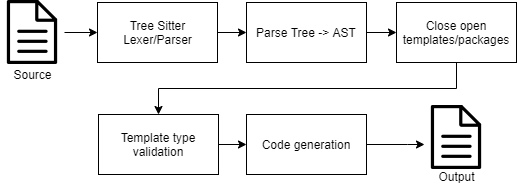
\includegraphics[scale=.75]{images/Compiler overview.png}
           \caption{Overview of the compiler}
           \label{fig:compiler-overview}
\end{figure}

\section{Lexer and Parser}\label{sec:lexer-and-parser}

\subsection{The PTS Grammar}\label{subsec:the-pts-grammar}

PTS is an extension of TypeScript, and the grammar is also therefore an extension of the TypeScript grammar.
There is no published official TypeScript grammar (other than interpreting it from the implementation of the TypeScript compiler), however up until recently there used to be a TypeScript specification\cite{tsspec}.
This TypeScript specification was deprecated as it proved a to great a task to keep updated, with the ever-changing nature of the language.
However, most of the essential parts are still the same.
The PTS grammar is therefore based on the TypeScript specification, and on the ESTree Specification\cite{estreespec}.

In figure~\vref{fig:pts-grammar} we can see the PTS BNF grammar.
This is not the full grammar for PTS, as I have only included any additions or changes to the original TypeScript/JavaScript grammars.
More specifically the non-terminal $\bnfpn{declaration}$ is an extension of the original grammar, where we also include package and template declarations as legal declarations.
The productions for non-terminals $\bnfpn{id}$, $\bnfpn{class declaration}$, $\bnfpn{interface declaration}$, and $\bnfpn{class body}$ are also from the original grammar.



\begin{figure}
    \begin{bnf*}
        \bnfprod{declaration}
            { \bnfsk \bnfor \bnfpn{package declaration} \bnfor \bnfpn{template declaration} }\\
        \bnfprod{package declaration}
            { \bnfts{package} \bnfsp \bnfpn{id} \bnfsp \bnfpn{PT body} }\\
        \bnfprod{template declaration}
            { \bnfts{template} \bnfsp \bnfpn{id} \bnfsp \bnfpn{PT body} }\\
        \bnfprod{PT body}
            { \bnfts{\{} \bnfsp \bnfpn{PT body decls} \bnfsp \bnfts{\}} }\\
        \bnfprod{PT body decls}
            { \bnfpn{PT body decls} \bnfsp \bnfpn{PT body decl} \bnfor \bnfes}\\
        \bnfprod{PT body decl}
            { \bnfpn{inst statement} \bnfor \bnfpn{addto statement} \bnfor }\\
        \bnfmore{ \bnfpn{class declaration} \bnfor \bnfpn{interface declaration} }\\
        \bnfprod{inst statement}
            { \bnfts{inst} \bnfsp \bnfpn{id} \bnfsp \bnfpn{inst rename block} }\\
        \bnfprod{inst rename block}
            { \bnfts{\{} \bnfsp \bnfpn{class renamings} \bnfsp \bnfts{\}} \bnfor \bnfes }\\
        \bnfprod{class renamings}
            { \bnfpn{class rename} \bnfor \bnfpn{class rename} \bnfts{,} \bnfsp \bnfpn{class renamings} }\\
        \bnfprod{class rename}
            { \bnfpn{rename} \bnfsp \bnfpn{field rename block} }\\
        \bnfprod{field rename block}
            { \bnfts{(} \bnfsp \bnfpn{field renamings} \bnfsp \bnfts{)} \bnfor \bnfes }\\
        \bnfprod{field renamings}
            { \bnfpn{rename} \bnfor \bnfpn{rename} \bnfts{,} \bnfsp \bnfpn{field renamings} }\\
        \bnfprod{rename}
            { \bnfpn{id} \bnfsp \bnfts{->} \bnfsp \bnfpn{id} }\\
        \bnfprod{addto statement}
            { \bnfts{addto} \bnfsp \bnfpn{id} \bnfsp \bnfpn{addto heritage} \bnfsp \bnfpn{class body} }\\
        \bnfprod{addto heritage}
            { \bnfpn{class heritage} \bnfor \bnfes }\\
    \end{bnf*}
    \caption{BNF grammar for PTS. The non-terminals $\bnfpn{declaration}$, $\bnfpn{id}$, $\bnfpn{class declaration}$, $\bnfpn{interface declaration}$, and $\bnfpn{class body}$ are productions from the TypeScript grammar.
    The ellipsis in the declaration production means that we extend the TypeScript production with some extra choices.}

    \textit{Legend:} Non-terminals are surrounded by $\bnfpn{angle brackets}$.
    Terminals are in $\bnfts{typewriter font}$.
    Meta-symbols are in regular font.
    \label{fig:pts-grammar}
\end{figure}


\subsection{Parser Generator}\label{subsec:parser-generator}

TypeScript is a language that is constantly updated, and is getting new features fairly often.


\begin{itemize}
    \item Preferably should allow us to change an existing grammar, without interfering with the original grammar, giving us the possibility to update the original grammar.
\end{itemize}

For our implementation of the grammar I choose to go with \href{https://tree-sitter.github.io/tree-sitter/}{Tree-sitter}.

Because
\begin{itemize}
    \item Lets you extend grammars
    \item Has JavaScript/Node API
    \item Makes it possible to use the grammar for syntax highlighting
\end{itemize}


As we talked about in section~\vref{sec:what-do-we-need}, we set ourselves the goal to find an approach that would allow us to create an implementation that was loosely coupled with TypeScript.
While a fork of the TypeScript compiler or the Babel parser would not allow this, Tree-sitter on the other hand allows extending existing grammars.
Extending a grammar works much like extending a class in an object-oriented language.
A "sub grammar" inherits all the rules from the "super grammar", so an empty ruleset would effectively work the same as the super grammar.
Just like most object-oriented languages have access to the super class, we also have access to the super grammar in Tree-sitter.
All of this enables us to add, override, and extend rules in an existing grammar, all while staying loosely coupled with the super grammar.
By extending the grammar, and not forking it, we are able to simply update our dependency on the TypeScript grammar, minimizing the possibility for conflicts.

where we have the ability to override rules from the super grammar with our own rules.
Not only are we able to override rules, but we can combine the old rules with the new.

A good example of overriding and combining rules can be found in the grammar of PTS, see listing~\vref{lst:overriding-combining-rule}, where we override the \codeword{\_declaration} rule from the TypeScript grammar, to include the possibility for package and template declarations.

\begin{code}{javascript}{Snippet from the PTS grammar, where we override the \codeword{\_declaration} rule from the TypeScript grammar, and adding two additional declarations.}{lst:overriding-combining-rule}
    _declaration: ($, previous) =>
        choice(
            previous,
            $.template_declaration,
            $.package_declaration
        )
\end{code}


\subsection{Instantiation and Renaming}\label{subsec:instantiation-and-renaming}

\subsubsection{Scoping}\label{subsubsec:inst-scoping}

For creating scopes I chose the following node types for "making new scopes".

\begin{itemize}
    \item \codeword{class\_body}
    \item \codeword{statement\_block}
    \item \codeword{enum\_body}
    \item \codeword{if\_statement}
    \item \codeword{else\_statement}
    \item \codeword{for\_statement}
    \item \codeword{for\_in\_statement}
    \item \codeword{while\_statement}
    \item \codeword{do\_statement}
    \item \codeword{try\_statement}
    \item \codeword{with\_statement}
\end{itemize}

\subsubsection{Transforming Nodes to Variable References}\label{subsubsec:transforming-nodes-to-variable-references}

\subsection{Verification of Templates}\label{subsec:verification-of-templates}

ts api

\subsection{Code Generation}\label{subsec:code-generation}

generate ts and compile ts to js through ts api.

\section{Notes on Performance}\label{sec:notes-on-performance}

Very slow compiler/PP because of the chosen implementation, with tree traverser for every step.


\section{Testing}\label{sec:testing}

\subsection{Lexer and Parser}\label{subsec:testing-lexer-and-parser}

Tree-sitter tests are simple \codeword{.txt} files split up into three sections, the name of the test, the code that should be parsed, and the expected parse tree in S-expressions\cite{sexprs}.

\begin{code}{typescript}{Example of tree-sitter grammar test}{lst:tree-sitter-grammar-test}
    ===========================
    Closed template declaration
    ===========================

    template T {
        class A {
            i = 0;
        }
    }

    ---
    (program
        (template_declaration
            name: (identifier)
            body: (package_template_body
                    (class_declaration
                        name: (type_identifier)
                        body: (class_body
                            (public_field_definition
                                name: (property_identifier)
                                value: (number)))))))

\end{code}

\subsection{Transpiler}\label{subsec:testing-transpiler}

Started with jest, and used some time to get it to work with typescript files, however had to switch because jest doesn't handle native libraries (tree-sitter) too well.
It \codeword{require}s the same native library several times, making the wrapping around the native program to break.